\cleardoublepage

\chapter{Conception de la solution}

%%%%%%%%%%%%%%%%%%%%%%%%%%%%%%%%%%%%%%%%%%%%%%%%%%%%%%%%%%%%%%%%%%%%%%%%%%%
%%%%%%%%%%%%%%%%%%%%%%%%%%%%%%%%%%%%%%%%%%%%%%%%%%%%%%%%%%%%%%%%%%%%%%%%%%%
%%%%%%%%%%%%%%%%%%%%%%%%%%%%%%%%%%%%%%%%%%%%%%%%%%%%%%%%%%%%%%%%%%%%%%%%%%%
%%%%%%%%%%%%%%%%%%%%%%%%%%%%%%%%%%%%%%%%%%%%%%%%%%%%%%%%%%%%%%%%%%%%%%%%%%%
%%%%%%%%%%%%%%%%%%%%%%%%%%%%%%%%%%%%%%%%%%%%%%%%%%%%%%%%%%%%%%%%%%%%%%%%%%%

\section{L'équipe du projet}

Pour réaliser ce projet, j'ai été intégré dans une petite équipe de trois personnes.

Un chef de projet qui est le relais entre Sopra Group et Limagrain afin d'établir la compréhension du besoin fonctionnel et technique.
Sa charge est d'une demi-journée par semaine.
De plus, il est chargé de la rédaction des spécifications de l'application.
Pour des raisons de délais trop courts et charges limitées, ces spécifications ont été réalisées en parallèle du développement, malgré l'éloignement des bonnes pratiques.

Un architecte qui a pour objectif de suivre le développeur, conseillant les outils, technologies et méthodes utilisées.
Sa charge sur le projet est aussi d'une demi-journée par semaine.

Et enfin moi-même, en tant que développeur, en charge du développement de l'application, à plein temps.

%%%%%%%%%%%%%%%%%%%%%%%%%%%%%%%%%%%%%%%%%%%%%%%%%%%%%%%%%%%%%%%%%%%%%%%%%%%
%%%%%%%%%%%%%%%%%%%%%%%%%%%%%%%%%%%%%%%%%%%%%%%%%%%%%%%%%%%%%%%%%%%%%%%%%%%
%%%%%%%%%%%%%%%%%%%%%%%%%%%%%%%%%%%%%%%%%%%%%%%%%%%%%%%%%%%%%%%%%%%%%%%%%%%
%%%%%%%%%%%%%%%%%%%%%%%%%%%%%%%%%%%%%%%%%%%%%%%%%%%%%%%%%%%%%%%%%%%%%%%%%%%
%%%%%%%%%%%%%%%%%%%%%%%%%%%%%%%%%%%%%%%%%%%%%%%%%%%%%%%%%%%%%%%%%%%%%%%%%%%

\section{La relation client}

%%%%%%%%%%%%%%%%%%%%%%%%%%%%%%%%%%%%%%%%%%%%%%%%%%%%%%%%%%%%%%%%%%%%%%%%%%%

\subsection{Assistance technique}

% TODO: détails assistance et différence avec projet (?)

Le projet s'est réalisé en mode \textit{assistance technique}.
Il n'y a aucune date de livraison imposée, par contre la charge (nombre de jours d'interventions) totale est fixe.

J'ai travaillé à raison de trois jours chez le client Limagrain et deux jours au siège de Sopra Group, profitant ainsi de la proximité du client pour éclaircir les points ambigus.

%%%%%%%%%%%%%%%%%%%%%%%%%%%%%%%%%%%%%%%%%%%%%%%%%%%%%%%%%%%%%%%%%%%%%%%%%%%

\subsection{Définition du besoin}

La relation directe avec le client m'a permis de définir le besoin du client au cours des différentes étapes du projet.

La première étape a consisté à établir le modèle de données.
Pour cela il a fallu étudier la solution existante pour déterminer les informations à mémoriser, leurs types, les contraintes, ainsi que les liens entre elles.
Cette partie est importante car la structure de l'application est fortement liée à ce modèle.

Deuxièmement, j'ai réalisé une première version de l'interface graphique de l'application.
L'objectif est de proposer une première maquette au client qui pourra effectuer des critiques.
L'ergonomie de la solution s'est ainsi optimisée au fur et à mesure des démonstrations.

Enfin, une fois l'application fonctionnelle, il était nécessaire d'importer les données existantes dans la nouvelle de données.
Comme ces deux bases de données sont différentes, il était nécessaire d'être en contact avec le client pour faire correspondre les schémas.

%%%%%%%%%%%%%%%%%%%%%%%%%%%%%%%%%%%%%%%%%%%%%%%%%%%%%%%%%%%%%%%%%%%%%%%%%%%
%%%%%%%%%%%%%%%%%%%%%%%%%%%%%%%%%%%%%%%%%%%%%%%%%%%%%%%%%%%%%%%%%%%%%%%%%%%
%%%%%%%%%%%%%%%%%%%%%%%%%%%%%%%%%%%%%%%%%%%%%%%%%%%%%%%%%%%%%%%%%%%%%%%%%%%
%%%%%%%%%%%%%%%%%%%%%%%%%%%%%%%%%%%%%%%%%%%%%%%%%%%%%%%%%%%%%%%%%%%%%%%%%%%
%%%%%%%%%%%%%%%%%%%%%%%%%%%%%%%%%%%%%%%%%%%%%%%%%%%%%%%%%%%%%%%%%%%%%%%%%%%

\section{Technologies et architecture}

Dans cette section je vous présenterai les différentes technologies utilisées dans le projet ainsi que leurs interactions.
La figure \ref{architecture} schématise les différents composants et communications.
\begin{figure}[!h]
	\center
	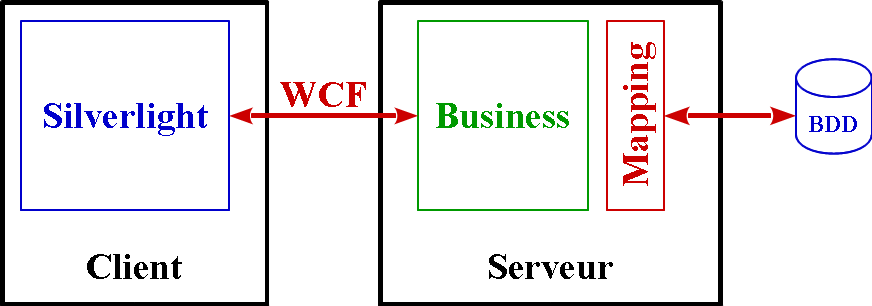
\includegraphics[width=0.8\textwidth]{img/architecture.png}
	\caption{Architecture du projet}
	\label{architecture}
\end{figure}
~~\\

Le groupe Limagrain travaille dans un environnement Microsoft et utilise ainsi leurs technologies et logiciels, comme par exemple : Windows pour le système d'exploitation, Internet Explorer comme navigateur internet, Outlook comme messagerie, \ldots

Pour développer cette solution nous nous sommes donc tournés vers les technologies Microsoft, facilitant ainsi la compatibilité et l'intégration des composants.
\\

L'architecture d'une application est importante, car cela définie sa maintenabilité et son évolutivité.
De plus cela permet la séparation des problèmes diminuant ainsi la complexité.

Notre application est divisée en 3 couches, appelée \textit{3-tiers}, qui est le modèle multi-tiers le plus utilisé.
Cela permet de séparer l'accès aux données de la base, la partie métier effectuant les traitements, et l'interface de l'utilisateur, comme le représente la figure \ref{architecture_3_tiers}.
\begin{figure}[!h]
	\center
	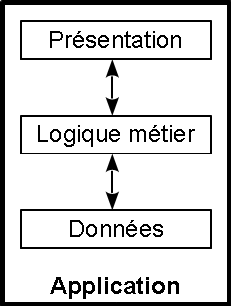
\includegraphics[width=0.4\textwidth]{img/architecture_3_tiers.png}
	\caption{Architecture 3 tiers}
	\label{architecture_3_tiers}
\end{figure}

%%%%%%%%%%%%%%%%%%%%%%%%%%%%%%%%%%%%%%%%%%%%%%%%%%%%%%%%%%%%%%%%%%%%%%%%%%%
%%%%%%%%%%%%%%%%%%%%%%%%%%%%%%%%%%%%%%%%%%%%%%%%%%%%%%%%%%%%%%%%%%%%%%%%%%%
%%%%%%%%%%%%%%%%%%%%%%%%%%%%%%%%%%%%%%%%%%%%%%%%%%%%%%%%%%%%%%%%%%%%%%%%%%%

\subsection{Socle}

% TODO: socle = framework ?
La solution développée se base sur un socle existant, développé dans le cadre d'un autre projet.
Ceci nous a permis un gain de temps important car une partie importante du projet n'a dû être développé à nouveau.
En contrepartie, les différentes technologies utilisées nous ont été imposées.

%%%%%%%%%%%%%%%%%%%%%%%%%%%%%%%%%%%%%%%%%%%%%%%%%%%%%%%%%%%%%%%%%%%%%%%%%%%

\subsubsection{Gestion des utilisateurs}

Le socle permet une gestion des utilisateurs de l'application.
Il est possible de les créer, modifier ou supprimer, pour restreindre l'accès aux personnes autorisées.
De plus, il est possible de connecter l'application à un LDAP.
\\

Le \textit{LDAP}, pour Lightweight Directory Access Protocol, est un protocole standard de gestion d'utilisateurs.
Son objectif est de centraliser les informations des utilisateurs (nom, identifiant, mot de passe, \ldots) dans un annuaire.

Le principal avantage de cette solution est la mise en commun des comptes utilisateurs, ce qui permet l'utilisation d'un seul et même compte pour tous les services connectés : Windows, la boite mail Outlook, cette application, \ldots

%%%%%%%%%%%%%%%%%%%%%%%%%%%%%%%%%%%%%%%%%%%%%%%%%%%%%%%%%%%%%%%%%%%%%%%%%%%

\subsubsection{Gestion des droits}

Il est aussi possible de gérer des droits dans l'application grâce à ce socle.
L'administrateur peut ainsi contrôler les accès et les actions des utilisateurs, protégeant ainsi les informations confidentielles.
\\

Chaque écran de l'application peut avoir leur accès ou certaines actions restreintes en fonction d'un \textit{droit}.
Ceux-ci peuvent prendre trois valeurs : 
\begin{itemize}
	\item "aucun accès", par défaut, qui interdit tout accès à l'écran ;
	\item "lecture" n'autorise que l'accès à l'écran, avec la possibilité d'effectuer des recherches ou d'afficher les détails ;
	\item "lecture et écriture" autorise toutes les actions possibles.
\end{itemize}

Un \textit{profil} est un ensemble de droits, qui permet de définir un périmètre d'action.
Par exemple un profil "administrateur" aura tous les droits dans l'application, un profil "manager" n'aura que des droits de lecture, ou encore un profil "ressources humaines" possèdera les droits liés aux candidats et contrats, \ldots

Chaque utilisateur possède un ou plusieurs profils, ce qui permet de définir l'ensemble de ses droits.
L'utilisation de profils, plutôt que de droit directement, permet un gain de temps.
En effet, l'administrateur des utilisateurs n'aura pas à affecter les nombreux droits aux nouveaux utilisateurs, et la modification d'un profil permet d'impacter l'ensemble des utilisateurs associés.
\\

La figure \ref{utilisateur_profils_droits} représente le schéma UML des utilisateurs, profils et droits dans l'application.
\begin{figure}[!h]
	\center
	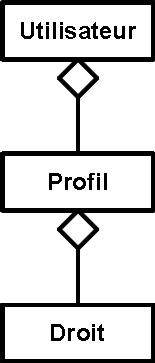
\includegraphics[width=0.2\textwidth]{img/utilisateur_profils_droits.png}
	\caption{Utilisation des profils et droits des utilisateurs}
	\label{utilisateur_profils_droits}
\end{figure}

%%%%%%%%%%%%%%%%%%%%%%%%%%%%%%%%%%%%%%%%%%%%%%%%%%%%%%%%%%%%%%%%%%%%%%%%%%%

\subsubsection{Programmation modulaire}
\label{Programmation modulaire}

Un module est un projet indépendant effectuant une tâche particulière.
Le socle offre la possibilité de programmer de façon modulaire, où chacun des modules ne possèdent (quasiment) aucune interaction entre elles.

Ainsi pour programmer de manière structurée, plusieurs modules distincts ont été développés.
Ceci permet de séparer l'implémentation de tâches distinctes.

%%%%%%%%%%%%%%%%%%%%%%%%%%%%%%%%%%%%%%%%%%%%%%%%%%%%%%%%%%%%%%%%%%%%%%%%%%%
%%%%%%%%%%%%%%%%%%%%%%%%%%%%%%%%%%%%%%%%%%%%%%%%%%%%%%%%%%%%%%%%%%%%%%%%%%%
%%%%%%%%%%%%%%%%%%%%%%%%%%%%%%%%%%%%%%%%%%%%%%%%%%%%%%%%%%%%%%%%%%%%%%%%%%%

\subsection{Langage de programmation}

%%%%%%%%%%%%%%%%%%%%%%%%%%%%%%%%%%%%%%%%%%%%%%%%%%%%%%%%%%%%%%%%%%%%%%%%%%%

\subsubsection{Microsoft .NET Framework}

\textit{.NET Framework} est une plateforme application proposée par Microsoft.
Cette technologie est comparable et directement concurrente de Java d'Oracle.

Ce framework est constitué de nombreux composants, disposés en couches au fur et à mesure de ses versions, schématisés sur la figure \ref{NET_Framework} :
\begin{enumerate}
	\item Le moteur d'exécution appelé Common Language Runtime (CLR) permet de compiler le code course en un langage intermédiaire appelé Microsoft Intermediate Language (MSIL).
Ce code est ensuite compilé à la volée lors de la première exécution grâce au compilateur "Just In Time" (JIT) ;
	\item Une bibliothèque de classes, offrant des fonctionnalités de base pour les différentes applications ;
	\item Plusieurs couches supplémentaires proposant des outils de développement d'interfaces graphique (WinForms), d'accès aux données (ADO.NET (Entity Framework)), \ldots
%	\item Une couche de trois composants : WinForms (ou Windows Forms) pour le développement d'interfaces graphiques, ASP.NET permettant la création de sites web dynamiques, et ADO.NET pour l'accès aux bases de données ;
%	\item La version 3.0 apporte Windows Presentation Foundation (WPF) permettant le développement d'applications graphiques vectorielles basées sur le XML, Windows Communication Foundation (WCF) pour la communication, Windows Workflow Foundation (WF) une technologie de gestion des workflow, et enfin Windows CardSpace pour la gestion d'identités ;
\end{enumerate}
\begin{figure}[!h]
	\center
	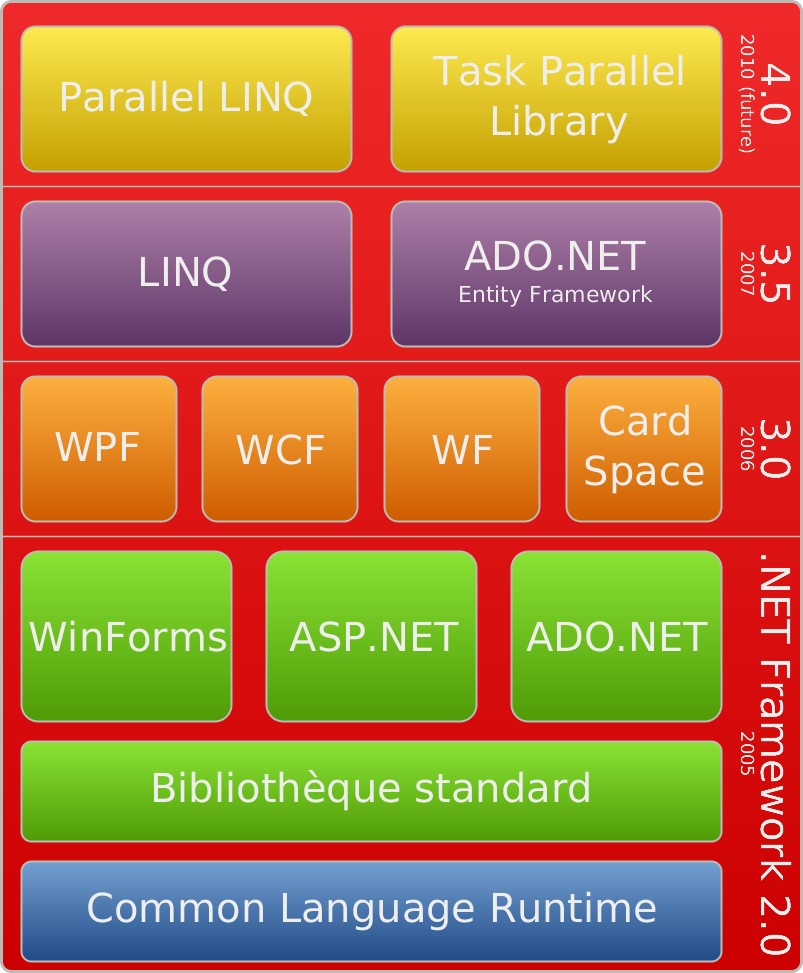
\includegraphics[width=0.6\textwidth]{img/NET_Framework.png}
	\caption{Couches de .NET Framework}
	Source : \href{http://fr.wikipedia.org/wiki/Framework\_.NET}{Wikipedia}
	\label{NET_Framework}
\end{figure}

%%%%%%%%%%%%%%%%%%%%%%%%%%%%%%%%%%%%%%%%%%%%%%%%%%%%%%%%%%%%%%%%%%%%%%%%%%%

\subsubsection{VB.NET}

\textit{Visual Basic .NET} est un langage de programmation développé par Microsoft.
Il s'agit d'une évolution majeure de Visual Basic 6, introduisant notamment l'aspect orienté objet.
De plus, le code est compilé dans le langage intermédiaire que les différents langages fonctionnant sur la machine virtuelle .Net.
Ce langage est très proche du C\#, à la syntaxe près.

Le projet a été développé dans ce langage, aussi bien la couche métier que la couche présentation.

%%%%%%%%%%%%%%%%%%%%%%%%%%%%%%%%%%%%%%%%%%%%%%%%%%%%%%%%%%%%%%%%%%%%%%%%%%%

\subsubsection{Apache log4net}

% TODO: pourquoi ce logger ?

Les \textit{log} sont les informations mémorisées lors du fonctionnement d'un programme informatique.
Ils permettent de garder des traces d'exécution, notamment lors du démarrage, de l'arrêt, ou d'erreurs.
Les log peuvent faciliter le débogage et la recherche d'anomalies.
Un ou plusieurs fichiers texte sont générés donnant accès à ces informations.

Le framework \textit{log4net}\footnote{log4net - Site web : \url{http://logging.apache.org/log4net/}} est un port sous Microsoft .NET du projet libre et open-source "Apache log4j".
Il permet de gérer simplement les log dans l'application.

%%%%%%%%%%%%%%%%%%%%%%%%%%%%%%%%%%%%%%%%%%%%%%%%%%%%%%%%%%%%%%%%%%%%%%%%%%%
%%%%%%%%%%%%%%%%%%%%%%%%%%%%%%%%%%%%%%%%%%%%%%%%%%%%%%%%%%%%%%%%%%%%%%%%%%%
%%%%%%%%%%%%%%%%%%%%%%%%%%%%%%%%%%%%%%%%%%%%%%%%%%%%%%%%%%%%%%%%%%%%%%%%%%%

\subsection{Base de données}

Une \textit{base de données} permet de stocker un grand nombre d'informations ayant des natures différentes.
Les données de même nature sont stockées dans des tables, où un champ possède un type et représente une valeur.

%%%%%%%%%%%%%%%%%%%%%%%%%%%%%%%%%%%%%%%%%%%%%%%%%%%%%%%%%%%%%%%%%%%%%%%%%%%

\subsubsection{PowerAMC}

\textit{PowerAMC}\footnote{PowerAMC - Site web : \url{http://www.sybase.fr/products/modelingdevelopment/poweramc}}, version francophone de PowerDesigner, est un logiciel de modélisation de bases de données produit par la société Sybase.
Il permet d'établir facilement un modèle de données à partir de son interface graphique, visible sur la figure \ref{PowerAMC}.
De plus, les scripts générés sont compatibles avec les différents types et versions de bases de données, ce qui permet de s'abstraire de certaines contraintes de compatibilité.
\begin{figure}[!h]
	\center
	
\includegraphics[width=0.9\textwidth]{img/PowerAMC.png}
	\caption{Interface de PowerAMC}
	\label{PowerAMC}
\end{figure}

Ce logiciel est utilisé par Sopra Group sur les différents projets.
Je l'ai donc utilisé sur ce projet.
Il m'a permis de concevoir, mais aussi d'effectuer les différentes modifications très simplement.

%%%%%%%%%%%%%%%%%%%%%%%%%%%%%%%%%%%%%%%%%%%%%%%%%%%%%%%%%%%%%%%%%%%%%%%%%%%

\subsubsection{SQL Server}

Il existe de nombreux systèmes de gestion de bases de données : Oracle, MySQL, PostgreSQL, \ldots Nous avons utilisé \textit{Microsoft SQL Server}, par demande du client car il s'agit d'un standard pour Limagrain.

%%%%%%%%%%%%%%%%%%%%%%%%%%%%%%%%%%%%%%%%%%%%%%%%%%%%%%%%%%%%%%%%%%%%%%%%%%%

\subsubsection{Mapping de la base de données}

\Jparagraph{Définition}

Le "modèle relationnel" est utilisé dans les systèmes de gestion de bases de données (SGBD) pour rassembler un ensemble d'informations.
Les données (clés) sont dupliquées entre les tables et l'accès aux relations s'effectue ensuite grâce à des jointures entre les tables.

Le "modèle objet", quant à lui, est utilisé dans la programmation orientée objet.
Les données sont modélisées sous la forme d'objets, entités complexes ayant des comportements et des relations entre elles.

Le \textit{mapping objet-relationnel} consiste à interfacer le modèle relationnel d'une base de données avec le modèle orienté objet d'un programme informatique.
Généralement, une classe modélisera une table, et attribut d'objet modélisera un champ d'une table, avec un type similaire (par exemple \lstinline{String} pour \lstinline{varchar}).


\Jparagraph{Entity Framework}

Cette opération peut être faite à l'aide d'un framework, permettant de s'abstraire de la base de données, automatisant et réduisant ainsi la duplication de code.
L'objectif est de faciliter le développement, augmenter la maintenabilité du programme, ou encore s'abstenir du type de bases de données.
Ainsi, la réaction, la recherche, la mise à jour ou la suppression (opérations CRUD) de données se font de manières simplifiées voir transparentes pour l'utilisateur.

Microsoft propose plusieurs framework, et c'est \textit{Entity Framework} qui a été utilisé.
Il est intégré à Visual Studio, ce qui permet une génération et un paramétrage facile d'utilisation.
De plus, il permet l'interaction avec  LINQ (Language-Integrated Query), extension du langage permettant de faire des requêtes sur des ensembles de données en s'abstrayant du type.

%%%%%%%%%%%%%%%%%%%%%%%%%%%%%%%%%%%%%%%%%%%%%%%%%%%%%%%%%%%%%%%%%%%%%%%%%%%
%%%%%%%%%%%%%%%%%%%%%%%%%%%%%%%%%%%%%%%%%%%%%%%%%%%%%%%%%%%%%%%%%%%%%%%%%%%
%%%%%%%%%%%%%%%%%%%%%%%%%%%%%%%%%%%%%%%%%%%%%%%%%%%%%%%%%%%%%%%%%%%%%%%%%%%

\subsection{Les services}

La couche de \textit{service} est la partie métier de l'application.
Elle permet de séparer le code source lié à l'affichage destiné à l'utilisateur, du code métier effectuant des traitements dans l'application.

%%%%%%%%%%%%%%%%%%%%%%%%%%%%%%%%%%%%%%%%%%%%%%%%%%%%%%%%%%%%%%%%%%%%%%%%%%%

\subsubsection{Client-Serveur}

\Jparagraph{Nécessité}

Il est nécessaire de faire communiquer la couche cliente de l'application avec la couche métier en raison de l'utilisation de Silverlight, comme je l'expliquerai dans la section \ref{Silverlight} ci-après.
Ces deux couches ne peuvent communiquer directement entre elles car l'une est exécutée sur le serveur et l'autre sur l'ordinateur de l'utilisateur.
La solution consiste à utiliser un service web.


\Jparagraph{Web service}

Un \textit{service web} (ou \textit{web service}) est un programme informatique permettant la communication et l'échange d'informations entre des systèmes hétérogènes et distribués (local, réseau, internet, \ldots), exposant des fonctionnalités.

L'échange d'informations entre le client et le serveur se fait par sérialisation, consistant à coder les informations contenues en mémoire.
Cela peut se faire sous le format texte (XML, JSON, \ldots) ou même sous format binaire.
L'objectif est d'échanger des données génériques et abstraites qui pourront être représentées dans n'importe quel langage.

L'exemple qui suit montre la sérialisation d'un même objet sous le format XML :
\begin{lstlisting}[language = xml]
<menu id="file" value="File">
	<popup>
		<menuitem value="New" onclick="CreateNewDoc()" />
		<menuitem value="Open" onclick="OpenDoc()" />
		<menuitem value="Close" onclick="CloseDoc()" />
	</popup>
</menu>
\end{lstlisting}
et JSON :
\begin{lstlisting}[language = sh]
{
	"menu": {
		"id": "file",
		"value": "File",
		"popup": {
			"menuitem": [
				{ "value": "New", "onclick": "CreateNewDoc()" },
				{ "value": "Open", "onclick": "OpenDoc()" },
				{ "value": "Close", "onclick": "CloseDoc()" }
			]
		}
	}
}
\end{lstlisting}


\Jparagraph{Windows Communication Foundation}

\textit{Windows Communication Foundation} [WCF], couramment appelé sous ses initiales WCF, est la couche de communication de .NET Framework, apparue dans la version 3.0.
Cette technologie respecte les normes standards des services web, ce qui lui permet d'appeler ou d'être appelé par des technologies différentes (Java, Python, \ldots).

Ce framework a été utilisé pour réaliser le service web de l'application, exposant ainsi différentes fonctions utiles à la couche d'affichage.

%%%%%%%%%%%%%%%%%%%%%%%%%%%%%%%%%%%%%%%%%%%%%%%%%%%%%%%%%%%%%%%%%%%%%%%%%%%

\subsubsection{WCF RIA Services}

Il est souvent nécessaire de posséder une logique applicative à la fois du côté serveur et du côté client.
C'est le cas par exemple lorsque l'on souhaite vérifier la validité des données avant de les insérer en bases de données :
\begin{enumerate}
	\item Soit on effectue la vérification côté serveur, impliquant l'échange inutile d'informations lorsque celles-ci sont fausses ;
	\item Soit la vérification est faite côté client, ce qui empêcherait le bon contrôle des flux d'entrée avant le traitement, ce qui pourrait amener à des erreurs ;
	\item Soit on effectue la même vérification à la fois du côté client et du côté serveur, mais cela impose de dupliquer le même code dans les deux couches.
\end{enumerate}
~~\\

Pour éviter ce problème, Microsoft propose le framework \textit{WCF RIA Services} [RIA].
Cet outil duplique du code d'un projet pour le copier dans un autre, de façon automatique lors de la compilation.
L'opération est schématisée sur la figure \ref{WCF_RIA_Services}.
Ceci permet d'avoir un code métier constamment à jour sans avoir à effectuer les modifications dans les différentes couches.
\begin{figure}[!h]
	\center
	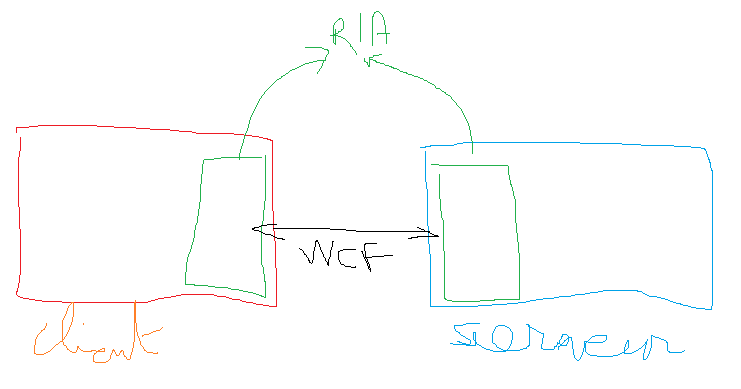
\includegraphics[width=1\textwidth]{img/WCF_RIA_Services.png}
	\caption{Fonctionnement de l'application client-serveur}
	\label{WCF_RIA_Services}
\end{figure}

%%%%%%%%%%%%%%%%%%%%%%%%%%%%%%%%%%%%%%%%%%%%%%%%%%%%%%%%%%%%%%%%%%%%%%%%%%%

\subsubsection{Reporting services}

Microsoft fournit un outil de génération de rapports appelé \textit{Reporting services}, intégré à la suite SQL Server.
Les fichiers source utilisés par le service se présentent sous la forme d'un fichier XML.
Visual Studio propose un éditeur graphique simplifiant son édition, la mise en forme ainsi que la création de requêtes.
\\

Le fonctionnement du service est représenté par la figure \ref{reporting_services} et se déroule en plusieurs étapes :
\begin{figure}[!h]
	\center
	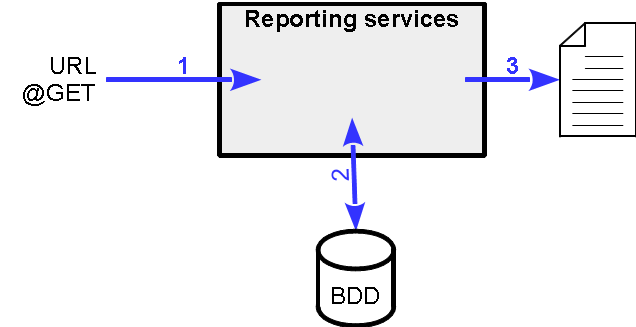
\includegraphics[width=0.9\textwidth]{img/reporting_services.png}
	\caption{Fonctionnement de reporting services}
	\label{reporting_services}
\end{figure}
\begin{enumerate}
	\item On appelle le service à l'aide de son adresse IP ou son nom de domaine.
Il est possible de passer des paramètres dans l'URL en utilisant la méthode GET.
Par exemple, si le service est accessible à l'URL \lstinline{http://nomserveur/reports/}, l'appel de \lstinline{http://nomserveur/reports/ID=5&name=toto} permet de spécifier les paramètres \lstinline{ID} et \lstinline{name} avec les valeurs respectives \lstinline{5} et \lstinline{toto}.
	\item Le serveur effectue les requêtes nécessaires dans la base de données afin de récupérer les données dynamiques du rapport.
	\item Le rapport est généré puis retourné au client au format HTML, PDF ou autre.
\end{enumerate}
~~\\

Ce type de service a été utilisé dans le projet.
Il est ainsi facile de générer les divers documents à imprimer avec les informations correspondantes aux contrats et candidats.
Le serveur de rapports est installé sur la même machine que celle de la base de données, pour ne pas avoir à installer inutilement SQL Server, mais aussi parce que tous les serveurs sont installés sur la même machine.

%%%%%%%%%%%%%%%%%%%%%%%%%%%%%%%%%%%%%%%%%%%%%%%%%%%%%%%%%%%%%%%%%%%%%%%%%%%
%%%%%%%%%%%%%%%%%%%%%%%%%%%%%%%%%%%%%%%%%%%%%%%%%%%%%%%%%%%%%%%%%%%%%%%%%%%
%%%%%%%%%%%%%%%%%%%%%%%%%%%%%%%%%%%%%%%%%%%%%%%%%%%%%%%%%%%%%%%%%%%%%%%%%%%

\subsection{Interface utilisateur}

%%%%%%%%%%%%%%%%%%%%%%%%%%%%%%%%%%%%%%%%%%%%%%%%%%%%%%%%%%%%%%%%%%%%%%%%%%%

\subsubsection{Silverlight}
\label{Silverlight}

\Jparagraph{Présentation}

Microsoft \textit{Silverlight} [Silverlight] est un plugin pour navigateur web.
Il permet le développement d'applications riches et de pousser plus loin l'expérience utilisateur du web 2.0, au même titre qu'Adobe Flash dont il se veut une alternative.
Initialement prévu pour des applications web dans un navigateur, les programmes peuvent être téléchargés pour être utilisés directement sur l'ordinateur ("out of browser"), et permettent aussi le développement d'applications pour Windows Phone 7.

Cette technologie nécessite l'installation du plugin, qui est un sous-ensemble de Microsoft .NET Framework.
Les applications sont ainsi cross-browser (Internet Explorer, Firefox, Chrome, \ldots) et cross-platform (Windows, mais aussi OS-X et Linux via le projet open-source Moonlight).
De plus les applications fonctionnent dans une "sandbox" ("bac à sable") ce qui permet de garantir une sécurité accrue pour l'utilisateur.

Une des spécifications de Silverlight est l'impossibilité d'appeler des services web de manière synchrone, c'est-à-dire que la fonction appelante attend la réponse.
En effet, lors d'un appel à un service le programme continue son exécution et un événement est émis lors de la réception de la réponse.
Cette solution permet de ne pas bloquer l'interface de l'utilisateur qui pourrait penser à un plantage de l'application.
Mais l'inconvénient est l'augmentation de la complexité de programmation car il est nécessaire de contrôler plusieurs fils d'exécution en parallèle.


\Jparagraph{Pattern MVVM}

Le pattern \textit{Modèle-Vue-VueModèle} a été créé par Microsoft a destination de Silverlight et Windows Presentation Foundation (WPF).
Il permet de structurer le développement d'interfaces graphiques en séparant la vue de la logique et de l'accès aux données, comme l'illustre le schéma de la figure \ref{MVVM}.
Le couplage est plus faible qu'avec le pattern Modèle-Vue-Contrôleur (MVC), ce qui permet une maintenance, une réutilisabilité et des tests plus faciles.
\begin{figure}[!h]
	\center
	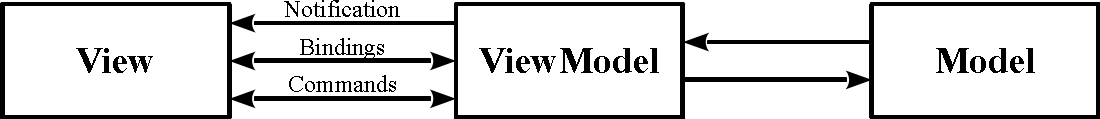
\includegraphics[width=1\textwidth]{img/MVVM.png}
	\caption{Pattern Modèle-Vue-VueModèle}
	\label{MVVM}
\end{figure}
~~\\

La vue du pattern MVVM utilise le langage \textit{XAML}, dérivé du langage XML, développé pour les besoins de Microsoft.
Son aspect générique sans code source permet aux interfaces graphiques d'être réutilisées dans diverses application et divers langages (C\#, VB.NET, \ldots).

L'exemple qui suit affiche une zone de saisie dont le contenu est bindé à la propriété \lstinline{PersonName} du ViewModel.
Ainsi une modification de la View mettra à jour automatiquement la propriété, et inversement une modification de la propriété du ViewModel mettra à jour la View.
\begin{lstlisting}[language = xml]
<Window xmlns="...">
	<TextBox Text="{Binding Path=PersonName}"/>
</Window>
\end{lstlisting}

%%%%%%%%%%%%%%%%%%%%%%%%%%%%%%%%%%%%%%%%%%%%%%%%%%%%%%%%%%%%%%%%%%%%%%%%%%%

\subsubsection{ASP.NET}

Un projet "Web Silverlight" nécessite la création d'un projet web, en plus du projet purement Silverlight.
En effet, ce projet web permet d'encapsuler le Silverlight pour le transmettre au navigateur du client.
Il est réalisé en \textit{ASP.NET} qui est une technologie Microsoft de programmation web, permettant de créer des sites dynamiques.

Il est nécessaire d'utiliser un serveur web pour déployer le projet ASP.NET.
Nous avons encore utilisé une technologie Microsoft : \textit{Internet Information Services}, plus couramment appelé \textit{IIS}.

%%%%%%%%%%%%%%%%%%%%%%%%%%%%%%%%%%%%%%%%%%%%%%%%%%%%%%%%%%%%%%%%%%%%%%%%%%%

\subsubsection{SignalR}

Le temps réel dans une application web permet au client de recevoir des données au moment où elles sont publiées.
Un exemple courant est une discussion instantanée : le serveur doit informer le client lors de la réception d'un message, sans que celui-ci n'ait à rafraichir la page continuellement.

Avant l'apparition du HTML5, il était nécessaire d'utiliser des techniques JavaScript en envoyant continuellement des requêtes du client vers le serveur.
Le HTML5 a apporté cette fonctionnalité grâce aux WebSocket, canal de communication bidirectionnel entre un navigateur web et un serveur web.

Microsoft fournit une bibliothèque intégrée à ASP.NET appelée \textit{SignalR}\footnote{SignalR - Site web : \url{http://signalr.net/}} permettant l'ajout de fonctionnalités de temps réel dans une application web.
Elle est basée sur les WebSocket et du JavaScript, facilitant ainsi son utilisation.